\resourceheading{6}{AAC Tool Selection and Implementation Guide}{Augmentative \& alternative communication\par}{Teachers, families, speech-language pathologists \& support teams}{Module 3 AAC Review, Grade 2 IGNITE curriculum, and TD Snap as a worked example}

\vspace{-0.5cm}
\toolsection{What This Resource Is}

This is a decision guide for evaluating an AAC tool as one part of a multimodal communication system. AAC includes aided and unaided methods, and eligibility should not depend on age, cognitive score, or mastery of prerequisite milestones \citep{ashaAAC,mirenda2015aids}. The core question is not whether a student can use a device in isolation, but whether the communicator can access meaningful vocabulary, participate across real routines, rely on responsive partners, and influence what happens next. TD Snap is the worked example because its current product information describes multiple page sets and access routes, including symbol-supported and text-based options, touch, switch scanning, and eye-gaze-compatible use \citep{tobii2026tdsnap}. Those features create possibilities; they do not replace individualized feature matching, trial use, training, technical support, funding review, or communicator consent. 
\begin{figure}[H]
\centering
\begin{tikzpicture}[
	node distance=0.06in,
	stage/.style={
		draw=DeepNavy,
		rounded corners=2pt,
		minimum width=1.22in,
		minimum height=0.34in,
		text width=1.12in,
		align=center,
		font=\tiny,
		inner sep=2pt
	},
	flow/.style={
		-{Latex[length=1.1mm]},
		line width=0.6pt,
		draw=PrimaryRed
	}
]

\node[font=\scriptsize\bfseries, text=DeepNavy] (title)
	{TD Snap in a Multimodal Communication System};

\node[stage, fill=SoftGold, below=0.07in of title] (intent)
	{\textbf{STUDENT MEANING}\\comment, question, refuse, repair};

\node[stage, fill=SoftBlue, right=of intent] (access)
	{\textbf{ACCESS ROUTE}\\touch, gaze, switch, gesture};

\node[stage, fill=SoftRose, right=of access] (tool)
	{\textbf{TOOL / DISPLAY}\\TD Snap, board, visual model};

\node[stage, fill=SoftGray, right=of tool] (partner)
	{\textbf{PARTNER}\\model, wait, notice, confirm};

\node[stage, fill=SoftGold, right=of partner] (agency)
	{\textbf{AGENCY}\\message changes what happens};

\draw[flow] (intent) -- (access);
\draw[flow] (access) -- (tool);
\draw[flow] (tool) -- (partner);
\draw[flow] (partner) -- (agency);

\node[
	draw=MidTeal,
	fill=SoftGreen,
	rounded corners=2pt,
	below=0.10in of tool,
	text width=6.25in,
	align=center,
	font=\tiny,
	inner sep=3pt
] (conditions)
{\textbf{Conditions that travel with the system:}
preference + consent $\bullet$ identity + language $\bullet$ low-tech backup $\bullet$ partner + technical support};

\node[
	draw=PrimaryRed,
	dashed,
	rounded corners=2pt,
	below=0.06in of conditions,
	text width=6.25in,
	align=center,
	font=\tiny,
	inner sep=3pt
] (equitas)
{\textbf{EQUITAS test:}
Can the student choose, refuse, comment, question, repair, revise, participate, and influence what happens next?
If not, revise the system---not the student.};

\end{tikzpicture}

\vspace{-0.05in}
\caption{\scriptsize
Communication becomes access-to-agency when meaning, access, tools, partners, and meaningful outcomes stay connected.}
\label{fig:td-snap-system}
\end{figure}

\vspace{-0.2in}
The same principle appeared in the Grade 2 IGNITE curriculum through shared visual models. In camp, students built a \textit{Before / During / After} pathway model to explain how tiny plastic pieces move through the environment and into living bodies. That artifact matters here because it shows that communication is not limited to speech or a single app: a student may comment, question, revise, point, explain, or co-construct meaning through a shared visual, partner prompting, gesture, writing, symbols, or a high-tech AAC system. AAC tool selection should therefore be judged by whether it expands participation and meaning-making, not by whether it makes a student look more conventionally verbal.

\toolsection{Shared Visual Model as a Communication Support}

\begin{center}
\begin{minipage}[c]{0.68\textwidth}
\centering
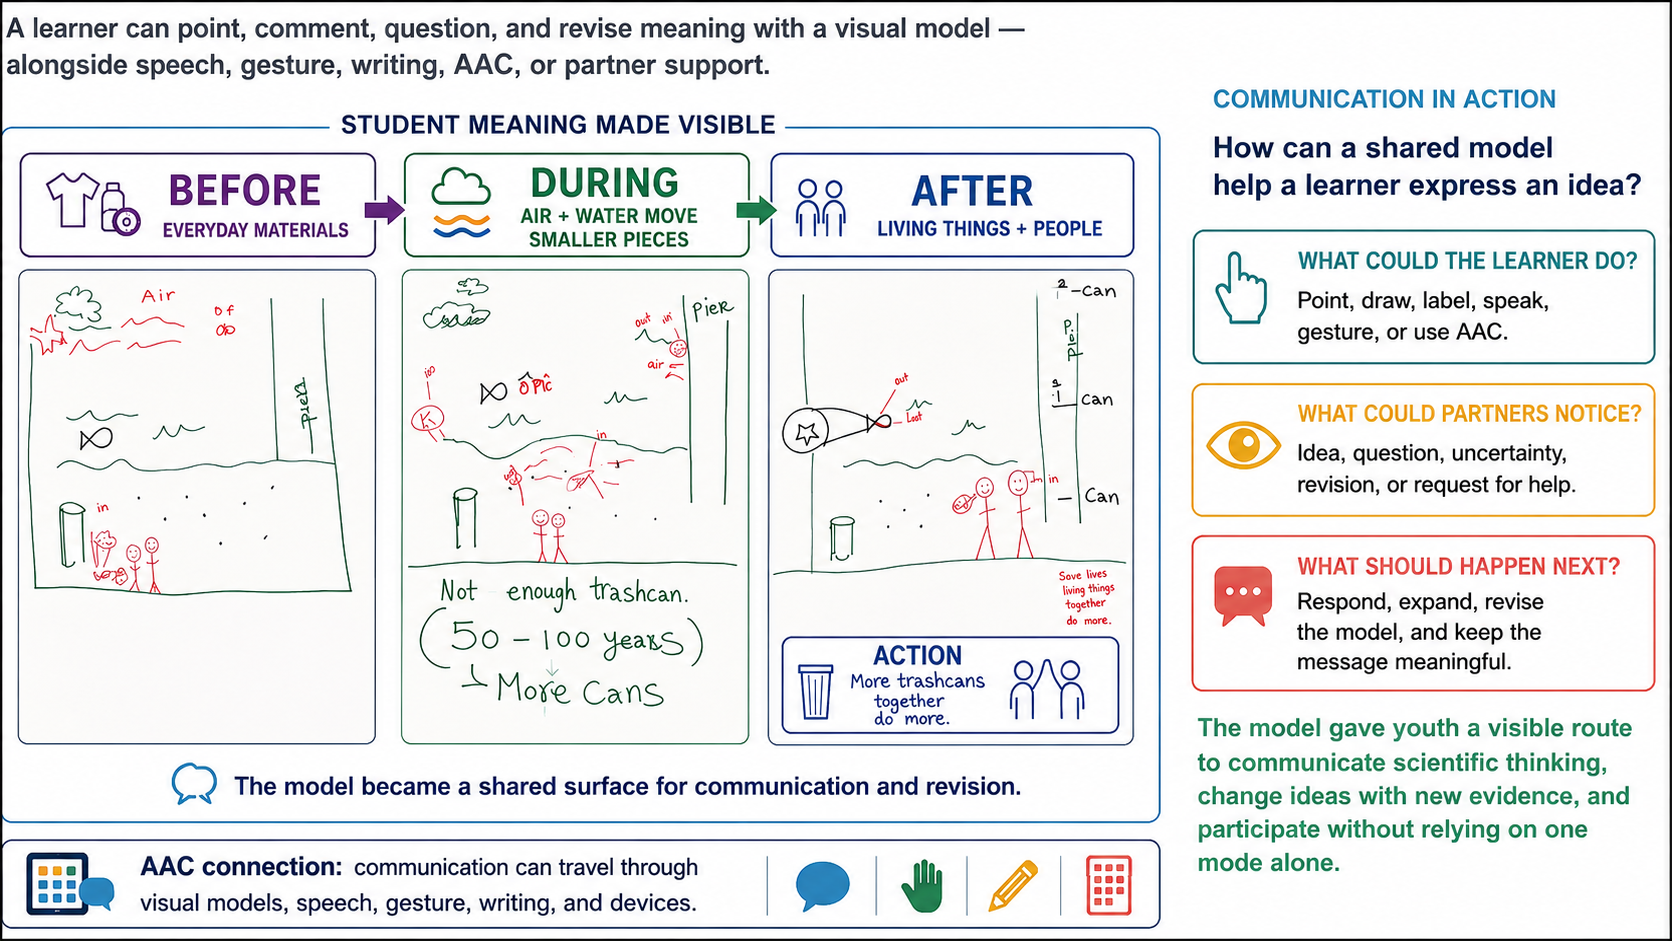
\includegraphics[
  width=1.0\linewidth,
  keepaspectratio
]{assets/artifact-previews/shared_visual_model_for_communication.png}
\end{minipage}
\hfill
\begin{minipage}[c]{0.29\textwidth}
\scriptsize

{\centering\bfseries\color{DeepNavy} Shared model, shared meaning.\par}
{\centering
The camp model functioned as a communication support because students could point to, revise, and explain ideas through a visible pathway rather than relying on speech alone. The three student-authored panels remained intact, while added prompts highlighted communicative purposes: naming the question, identifying what they thought, deciding what evidence was needed, and stating what should change.\par
}

{\centering
This makes the visual relevant to AAC: it supported commenting, questioning, revising, and action-planning through multiple response routes.\par
}
\end{minipage}
\end{center}




\newpage
\toolsection{AAC Selection and Trial Matrix}

\small
\renewcommand{\arraystretch}{1.0}
\setlength{\tabcolsep}{4pt}

\begin{longtable}{
>{\bfseries\RaggedRight\arraybackslash}p{1.0in}
>{\RaggedRight\arraybackslash}p{3.00in}
>{\RaggedRight\arraybackslash}p{2.87in}}

\tableheaderthree{Domain}{Questions for the Team}{Evidence During Trial}

Communicator &
What modes, languages, identities, interests, relationships, and messages matter now? What does the person accept, choose, or reject? &
Initiations, message range, preference, fatigue, refusal, repair, and whether the learner chooses among available communication routes \\

\rowcolor{SoftGray}
Access &
What routes are usable: touch, pointing, eye gaze, switch, scanning, gesture, positioning, vision, hearing, sensory, or motor access? &
Accuracy and effort across locations, materials, body positions, time of day, and changing access needs \\

Vocabulary \& representation &
Are core, activity, identity, bilingual, academic, social, humor, refusal, pain, and repair language available? Can meaning also be supported through symbols, photos, text, or shared visual models? &
The learner comments, questions, refuses, repairs, and revises ideas rather than using the system only to make requests \\

\rowcolor{SoftGray}
Partners &
Who models, waits, notices, confirms, repairs, and responds? Can partners recognize meaning across modes without replacing the learner's message? &
Adults reduce repeated prompts, recognize multiple communication routes, and allow messages to change what happens next \\

Continuity &
Will communication remain available through class, lunch, transitions, home, hands-on work, and device failure? &
High-tech, low-tech, and shared visual routes remain available; vocabulary and communication supports stay predictable \\

\rowcolor{SoftGray}
Outcome &
Does communication increase access, relationships, learning, privacy, choice, and influence? &
More self-initiated contributions and message functions---not simply more device activations
\end{longtable}

\vspace{-0.5cm}
\normalsize
\toolsection{Implementation Commitments}

Keep communication supports within reach; model without demanding imitation; pause for processing; accept pointing, gesture, writing, drawing, shared visual models, objects, and AAC as meaningful communication; confirm rather than assume; never remove AAC as punishment; and honor refusal and correction when safety permits. Program vocabulary with the communicator rather than limiting the system to adult-selected requests or behavior-management phrases. Most importantly, respond to the message: communication becomes consequential when a question, refusal, correction, preference, or new idea can change what happens next. Norrie, Waller, and Hannah show that AAC adoption depends on technical support, training, staffing, coordination, and daily context \citep{norrie2021context}. A device left on a shelf, removed during transitions, or used only with one specialist represents implementation failure.

\reflectionbox{\textbf{Practice-to-trial connection:} The Grade 2 IGNITE curriculum repeatedly plans for picture cards, speech devices, gestures, choice boards, visual schedules, step-by-step checklists, adaptive keyboards, speech-to-text, and voice recording within coding, building, and digital-storytelling tasks \citep{placement2026robotics}. EDU486 camp extended the same principle through pointing, drawing, photographing, partnering, passing, returning, and the shared \textit{Before / During / After} model. Youth could add, point to, question, and revise visible ideas as evidence changed. These artifacts identify real routines and communication demands for feature matching; they do \emph{not} establish that a particular learner or camper used TD Snap. A trial would test whether the selected system expands authorship within those existing communication routes.}

\adaptationbox{A feature-rich device or polished visual support can still narrow agency if adults change layouts frequently, omit bilingual or identity vocabulary, require device repetition after a clear message in another mode, or prioritize speed over authorship. Review the trial with the communicator and family. If access, meaning, or influence does not improve, revise the page set, access method, vocabulary, visual support, or partner practice rather than blaming the learner.}

\sourcebox{\scriptsize ASHA AAC overview \citep{ashaAAC}; multimodal AAC design \citep{mirenda2015aids}; context and adoption \citep{norrie2021context}; TD Snap product information \citep{tobii2026tdsnap}.}